\chapter{Anwendung statistischer Methoden}
\label{chapter:3}

In diesem Kapitel werden mehrere Programmiersprachen vorgestellt, die sich für Regressionsanalyse eignen. Dabei betrachten wir für Statistik entwickelte Programmiersprachen ebenso wie Software-Bibliotheken für maschinelles Lernen. Im letzten Teil dieses Kapitels wird demonstriert, wie man Regression mit vorhandener SQL-Syntax umsetzen und durchführen kann.

\section{Beispieldaten}
\label{section:3:1}

Wir arbeiten in dieser Arbeit mit Beispieldaten, welche mit einem Python-Skript erstellt wurden. Das Skript ist als Ganzes im Anhang \ref{appendix:A} zu finden. Die Daten liegen in Form einer csv-Datei vor, welche in so gut wie jeder Sprache einfach eingelesen werden kann.

Wir betrachten hier fiktive Kunden eines Onlinehandels. Für jeden Kunden wissen wir das Alter, die Anzahl seiner Käufe, die Summe des ausgegebenen Geldes und ob der Kunde eine Premium Mitgliedschaft besitzt oder nicht. Der ausgegebene Betrag wird in Cent angegeben, um mit ganzen Zahlen rechnen zu können. Die Premium-Mitgliedschaft wird mit einer 1 symbolisiert, während eine 0 das Gegenteil bedeutet.

Insgesamt wurden für diese Arbeit 100.000 solcher Datensätze erzeugt. Die Ergebnisse später dargestellten Ergebnisse wurden mit den ersten 1.000 Datenpunkten berechnet. In der folgenden Tabelle sind die ersten 10 dieser Datensätze dargestellt.

\begin{center}
  \captionof{table}{Auszug aus den Beispieldaten}
  \begin{tabular}{|c|c|c|c|}\hline
    \textbf{age} & \textbf{purchases} & \textbf{money} & \textbf{premium} \\ \hline
    30 & 1 & 4421 & 0 \\ \hline
    30 & 11 & 23346 & 1 \\ \hline
    33 & 1 & 4010 & 0 \\ \hline
    31 & 19 & 52517 & 1 \\ \hline
    29 & 3 & 8046 & 0 \\ \hline
    28 & 12 & 25295 & 0 \\ \hline
    41 & 16 & 38236 & 1 \\ \hline
    23 & 3 & 7098 & 1 \\ \hline
    25 & 1 & 2707 & 0 \\ \hline
    38 & 20 & 50976 & 1 \\ \hline
  \end{tabular}
\end{center}

Wir definieren uns außerdem drei Fragestellungen, welche wir mit den in Kapitel 2 vorgestellten Arten von Regressionen beantworten werden:
\begin{enumerate}
  \item Als Erstes wollen wir wissen, ob das ausgegebene Geld mit der Anzahl der Käufe in linearem Zusammenhang steht. Diese Fragen können wir mit einfacher linearer Regression beantworten. $money$ ist hierbei die abhängige Variable und $purchases$ ist die unabhängige Variable.
  \item Die zweite Frage ist ähnlich der Ersten. Hier wollen wir wissen, ob neben der Anzahl der Käufe auch das Alter des Kunden einen Einfluss auf das ausgegebene Geld hat. Hier haben wir nun zwei unabhängige Variablen, nämlich $age$ und $purchases$. Die abhängige Variable bleibt $money$. Diese Frage beantworten wir mit multipler linearer Regression.
  \item Zuletzt interessiert uns, ob eine Premium-Mitgliedschaft von der Summe des ausgegebenen Geldes zusammenhängt. $money$ ist also nun die unabhängige Variable, während $premium$ die abhängige Variable ist. Nachdem $premium$ eine binäre Variable ist, nutzen wir hier logistische Regression.
\end{enumerate}

\section{R-Projekt}
\label{section:3:2}

Das R-Projekt oder einfach nur R ist eine Sprache für statistische Berechnungen und graphische Darstellung. Damit ist R wie geschaffen für Regressionsanalyse.

\subsection{Grundprinzip}
\label{subsection:3:2:1}

In R sind Datenstrukturen wie Vektoren, Matrizen und Listen als Datentypen vorhanden. Darauf aufbauend existieren sogenannten Dataframes. Ein Dataframe ist eine Liste von Vektoren der gleichen Länge und wird in R zur Repräsentation von Datentabellen verwendet. Die Vektoren der Liste entsprechen den Attributen einer Relation. In einen solchen Dataframe importieren wir als erstes immer die Beispieldaten aus der csv-Datei.

In R lassen sich außerdem sogenannte Modelle definieren, welche als Eingabe nur die Daten und eine Formel benötigen. Eine Formel ist ein String der Form "$y \sim modell$" und symbolisiert den funktionalen Zusammenhang zwischen der abhängigen und den unabhängigen Variablen.

Hat man ein Modell erstellt, so bietet R Funktionen, um die Parameter für das gegebene Modell mittels Regressionsanalyse zu berechnen. Wir werden im Folgenden von den Funktionen $lm$ (für "linear model") und $glm$ (für "generalized linear model") Gebrauch machen.

\subsection{Einfache lineare Regression}
\label{subsection:3:2:2}

Betrachten wir also Frage Nummer $1$ aus dem vorherigen Teilkapitel. Die Formel lautet hier "$money \sim purchases$". Man liest also die Daten aus der csv-Datei, erstellt das Modell mit der genannten Formel und berechnet die Parameter mit der Funktion $lm$. Mit nur drei Zeilen Code lässt sich also die komplette Regressionsanalyse implementieren. Die print-Funktion dient zur Ausgabe des Ergebnisses.

\begin{minted}[linenos,breaklines,frame=single]{r}
  data <- read.csv2("sample.csv", sep = ",", header = TRUE)
  modell <- as.formula("money ~ purchases")
  slr <- lm(modell, data = data)
  print(slr)
\end{minted}

Das Ergebnis des obigen Codes ist folgendes:

\begin{minted}[linenos,breaklines,frame=single]{r}
  Coefficients:
  (Intercept)    purchases
      -150.5       2519.8
\end{minted}

Der Wert unter "$(Intercept)$" entspricht dabei dem Paramter $\alpha$ in unserer Notation, der Wert unter "$purchases$" entspricht $\beta$.

Der kleine Wert für $\alpha$ entspricht der Intuition, dass ein Kunde ohne Käufe auch kein Geld ausgegeben hat. Der relativ große Wert von ca. $2500$ für $\beta$ zeigt, dass die Anzahl der gekauften Artikel sehr einen großen Einfluss auf das ausgegebene Geld hat. Ein Kunde gibt pro gekauftem Artikel etwa $2500$ Cent, also $25$ Euro aus.

R verfügt auch über Möglichkeiten zur graphischen Darstellung. Lässt man die die Datenpunkte und die lineare Ausgleichsfunktion mit den berechneten Parameter plotten, erhält man dieses Diagramm:

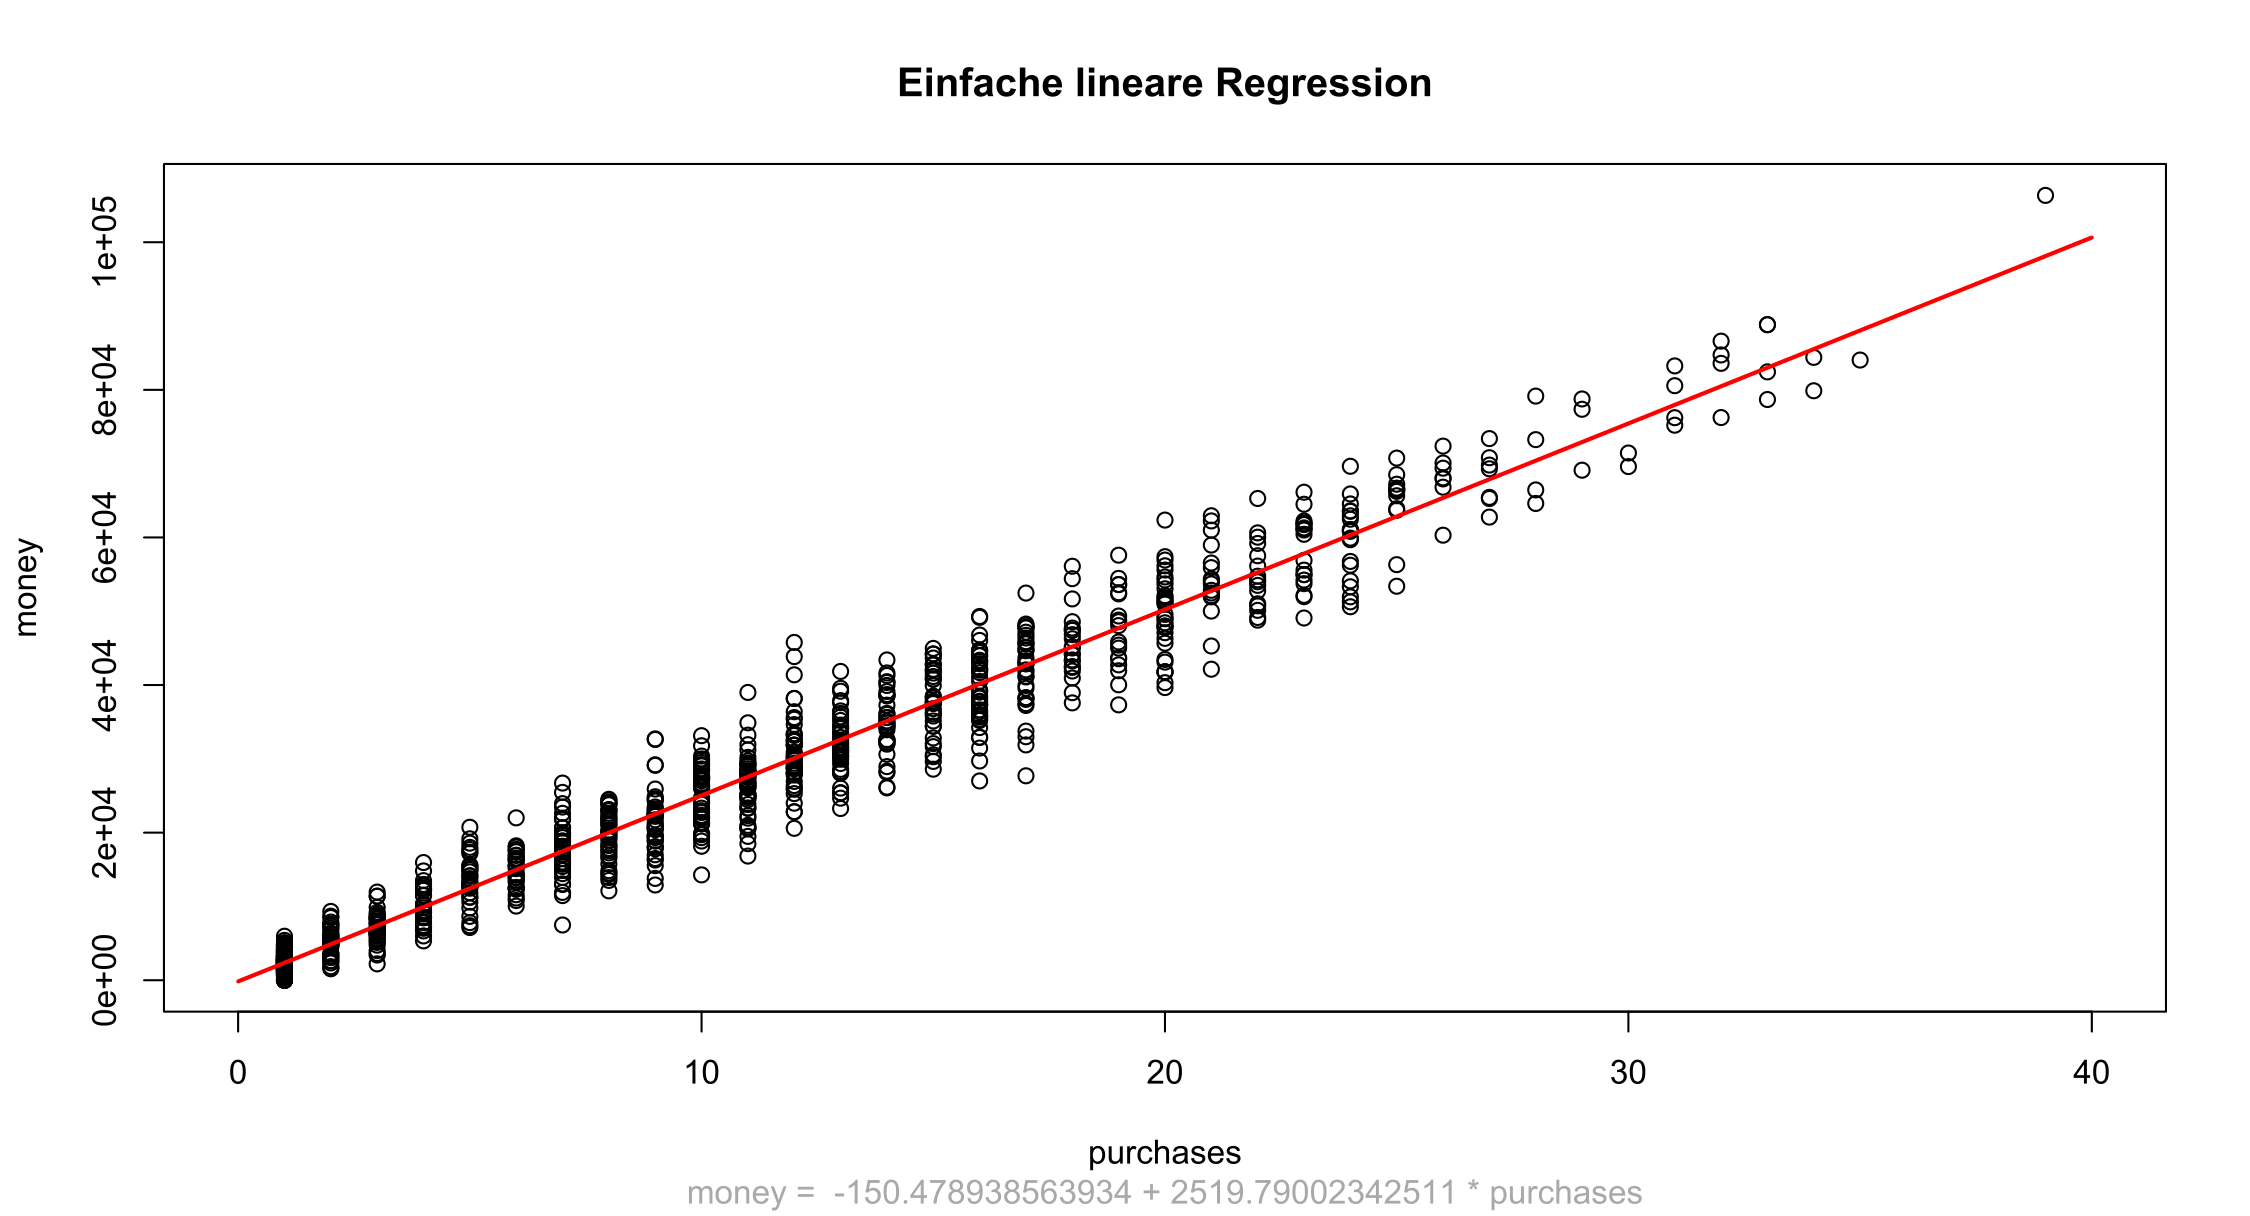
\includegraphics[width=\textwidth]{r-simpleLinearRegression}

\subsection{Multiple lineare Regression}
\label{subsection:3:2:3}

Bei multipler lineare Regression unterscheidet sich der R-Code nur in der Wahl der Formel von dem Code aus dem vorherigen Teilkapitel. Hier wollen wir $money$ durch eine lineare Summe von $purchases$ und $age$ modellieren, deshalb lautet die Formel hier "$money \sim purchases + age$". Man erhält hier das folgende Ergebnis.

\begin{minted}[linenos,breaklines,frame=single]{r}
  Coefficients:
  (Intercept)    purchases          age
       -766.7       2520.3         17.5
\end{minted}

Der Wert für $\alpha$ ist wieder relativ klein, der Wert für das $\beta$ zu $purchases$ ist fast exakt derselbe wie bei einfacher linerarer Regression, was bei denselben Daten auch zu erwarten war. Der Wert für das $\beta$ zu $age$ ist dagegen nahe bei null. Das bedeutet, dass das Alter im Vergleich zu der Anzahl der Käufe keinen signifikanten Einfluss auf das ausgegebene Geld hat.

\subsection{Logistische Regression}
\label{subsection:3:2:4}

Bei logistischer Regression nutzen wir nun nicht mehr ein lineares Modell wie bisher, sondern ein generalisiertes lineares Modell. Logistische Regression ist im Wesentlichen ein Spezialfall dieses Modelles. Hier nutzen wir also die $glm$-Funktion. Um logistische Regression damit betreiben zu können, wählt man den Parameter $family$ dieser Funktion als $binomial$.

Man braucht wie auch bei linearer Regression ein Formel für das Modell. Diese bildet man analog wie bisher, indem mal die abhängige Variable mit den unabhängigen Variablen über eine Tilde verbindet. Im Fall unserer dritten Fragestellung wählt man also die Formel als "$premium \sim money$".

Der gesamte R-Code für die logistische Regression ist wieder ähnlich zu dem Code aus \ref{subsection:3:2:1} und lautet wie folgt:

\begin{minted}[linenos,breaklines,frame=single]{r}
  data <- read.csv2("sample.csv", sep = ",", header = TRUE)
  modell <- as.formula("premium ~ money")
  logit <- glm(modell, family = binomial, data = data)
  print(logit)
\end{minted}

Nach der Ausführung erhält man das folgende Ergebnis:

\begin{minted}[linenos,breaklines,frame=single]{r}
  Coefficients:
  (Intercept)        money
   -1.9910911    0.0000803

  Degrees of Freedom: 999 Total (i.e. Null);  998 Residual
  Null Deviance:	    1386
  Residual Deviance: 1006 	AIC: 1010
\end{minted}

Eine anschauliche Interpretation der zurückgegebenen Parameter ist nicht mehr so einfach. Wir lassen uns das Ergebnis daher wieder als Plot visualisieren:

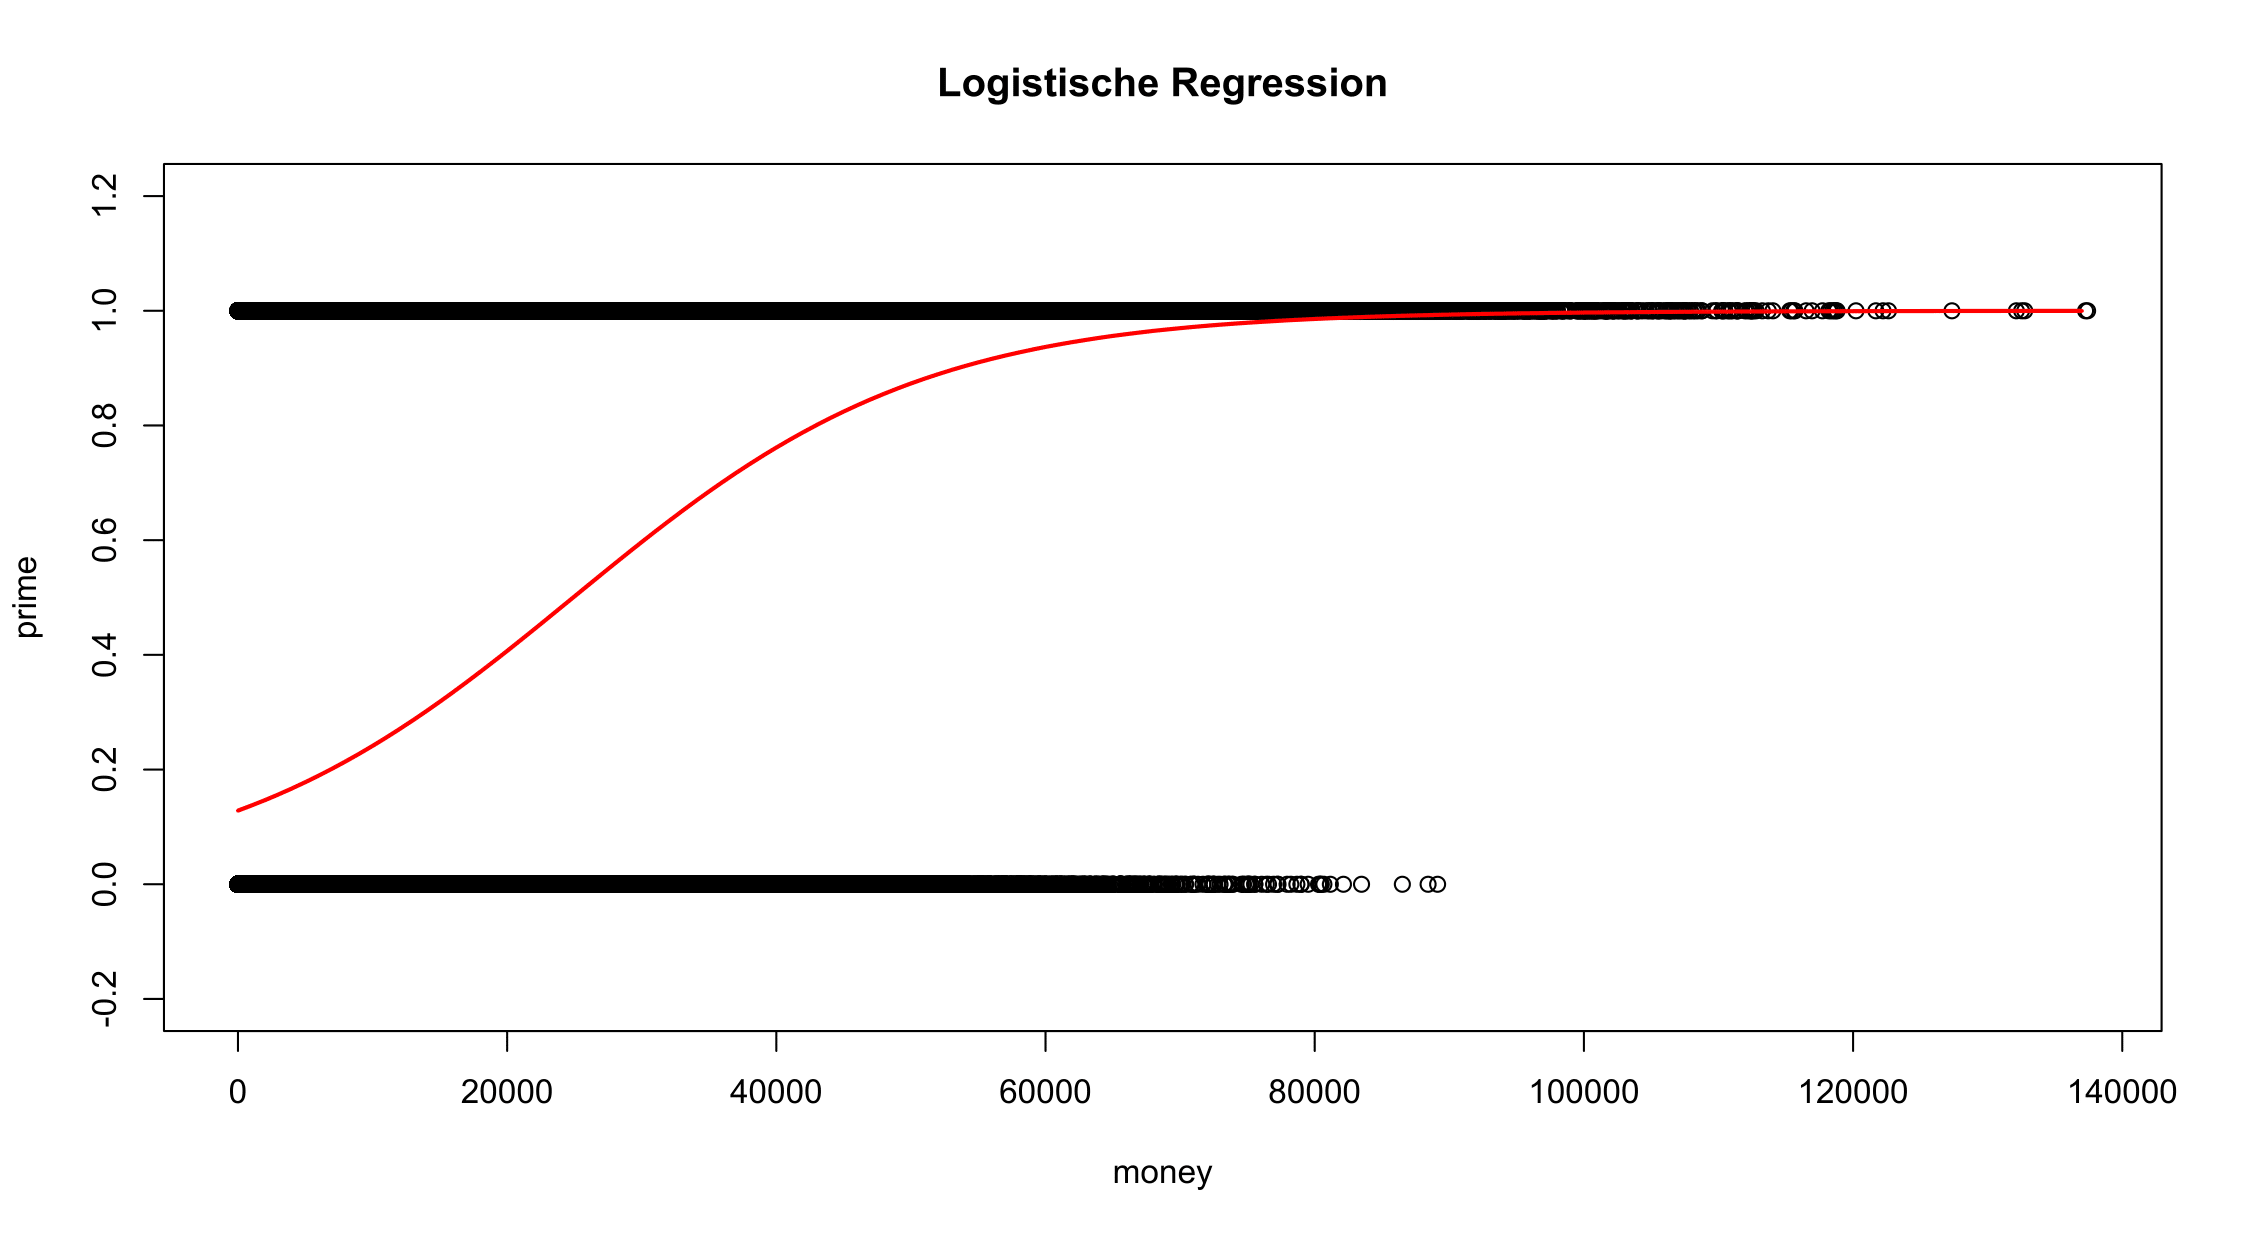
\includegraphics[width=\textwidth]{r-logisticRegression}

Für Kunden, die weniger als $100$ Euro ausgegeben haben ist die Wahrscheinlichkeit Premium-Mitglied zu sein mit etwa $25\%$ relativ gering. Je höher die Summe aber wird, desto größer wird auch die genannte Wahrscheinlichkeit. So ist ein Kunde mit mehr als $800$ Euro Ausgaben so gut wie immer ein Premium-Mitglied.

\section{TensorFlow}
\label{section:3:3}

TensorFlow ist eine Software-Bibliothek, die von Google für die Umsetzung von Algorithmen für maschinelles Lernen entwickelt wurde. Das umfasst insbesondere auch die Möglichkeit zur iterativen Optimierung von Kostenfunktionen, was wir nun zur Regressionsanalyse nutzen wollen.

TensorFlow bietet APIs für verschiedene Programmiersprachen an. Die Skripte, welche für dieser Arbeit erstellt wurden, sind in Python geschrieben. Wir verwenden TensorFlows Implementierung eines Gradientenabstiegsverfahrens, für welches man die Anzahl der Schritte und die Abstiegsgeschwindigkeit selbst wählen muss. Die Genauigkeit des Ergebnisses hängt also zusätzlich von einer angemessenen Auswahl dieser Werte ab.

Die Python-Skripte umfassen nun zwischen 70 und 100 Codezeilen, daher findet man diese Skripte im Ganzen nur im Anhang \ref{appendix:B}. Die wichtigsten Ausschnitte aus dem Code sollen in den folgenden Teilkapiteln aber einen Einblick in die Funktionsweise des Codes geben.

\subsection{Grundprinzip}
\label{subsection:3:3:1}

TensorFlow arbeitet mit Tensoren als grundliegende Datenstruktur. Solche sind im Wesentlichen Matrizen mit festen Dimensionen. Tensoren können dann mit Hilfe verschiedenster Operatoren weiterverarbeitet werden.

Es gibt drei Möglichkeiten, Tensoren zu definieren: Als Konstante, als Variable oder als Platzhalter. Während Konstanten ihren Wert nicht mehr ändern können, sind die beiden letztgenannten veränderbar. Der Unterschied besteht darin, dass Variablen mit einem Startwert initiiert werden, Platzhalter besitzen dagegen anfangs keinen Wert. Wir werden Variablen nutzen, um die Parameter über die Iterationen zu speichern. Die Daten, mit denen wir das Modell trainieren werden, übergeben wir an Platzhalter.

Wie das Modell exakt definiert wird, zeigen die folgenden Teilkapitel. Wir stellen immer eine Kostenfunktion auf, die dann mit Hilfe eines Gradientenabstiegsverfahrens iterativ minimiert wird. Die Definition dieses sogenannten Trainingsschrittes sieht immer gleich aus:

\begin{minted}[linenos,breaklines,frame=single]{python}
  train_step = tf.train
                 .GradientDescentOptimizer(learn_rate)
                 .minimize(cost)
\end{minted}

Dabei ist $tf$ die importierte TensorFlow-Bibliothek, $learn\_rate$ ist die Geschwindigkeit bzw. Schrittweite des Verfahrens und $cost$ ist die zuvor definierte Kostenfunktion.

Um dann auch wirklich Berechnungen durchführen zu können, muss in TensorFlow eine Session erzeugt werden. In dieser Session wird dann die Iteration gestartet, die $train\_step$ immer wieder mit echten Daten füttert. Je mehr Iterationen durchlaufen werden, desto exakter werden die Parameter berechnet.

\subsection{Einfache lineare Regression}
\label{subsection:3:3:2}

Hier definieren wir unsere Platzhalter und Variablen wie folgt:

\begin{minted}[linenos,breaklines,frame=single]{python}
  x = tf.placeholder(tf.float32, [None, 1])
  y = tf.placeholder(tf.float32, [None, 1])
  alpha = tf.Variable(tf.zeros([1]))
  beta = tf.Variable(tf.zeros([1, 1]))
\end{minted}

$x$ und $y$ sind die Platzhalter für die Beispieldatensätze für das später folgende Training. $alpha$ und $beta$ sind die Parameter-Variablen, welche mit Werten null initiiert werden. Daraus berechnen wir über den linearen funktionalen Zusammenhang die geschätzten $y$ Werte:

\begin{minted}[linenos,breaklines,frame=single]{python}
  y_calc = tf.matmul(x, beta) + alpha
\end{minted}

Die Funktion $tf.matmul$ führt Matrizenmultiplikation durch. Nun definieren wir noch die Kostenfunktion als Mittelwert der Quadrate zwischen den wahren und geschätzten $y$-Werten:

\begin{minted}[linenos,breaklines,frame=single]{python}
  cost = tf.reduce_mean(tf.square(y - y_calc))
\end{minted}

Damit können wir die Session starten und unsere Parameter berechnen lassen. Mit einer Schrittweite von $0.0054$ und $2000$ Iterationen erhält man folgendes Ergebnis:

\begin{minted}[linenos,breaklines,frame=single]{python}
  alpha:  -150.377670
  beta:   2519.784424
  cost:   15031988.000000
\end{minted}

Die hier berechneten Werte für $alpha$ und $beta$ sind schon sehr nahe an den exakten Werten. Zusätzlich geben wir hier auch den aktuellen Wert der Kostenfunktion aus.

\subsection{Multiple lineare Regression}
\label{subsection:3:3:3}

Nachdem in diesem Fall nun mehr unabhängige Variablen vorhanden sind, vergrößern wir die Dimension der Tensoren $x$ und $beta$ um eins.

\begin{minted}[linenos,breaklines,frame=single]{python}
  x = tf.placeholder(tf.float32, [None, 2])
  beta = tf.Variable(tf.zeros([2, 1]))
\end{minted}

Die restlichen Variablen werden wie bei einfacher linearer Regression definiert. Das Gradientenverfahren ist bei zwei abhängigen Variablen nun komplexer, daher muss die Schrittweite verringert werden. Eine Folge davon ist, dass man mehr Schritte für dieselbe Präzision des Ergebnisses durchführen muss. Bei einer Schrittweite von $0.00071$ und $50000$ Schritten erhält man folgendes Ergebnis:

\begin{minted}[linenos,breaklines,frame=single]{python}
  alpha:           -754.910095
  beta_purchases:  2520.172363
  beta_age:        17.224550
  cost:            15004541.000000
\end{minted}

\subsection{Logistische Regression}
\label{subsection:3:3:4}

Wir definieren unsere Tensoren exakt wie bei einfacher linearer Regression, da wie hier wieder mit je einer unabhängigen und einer abhängigen Variablen arbeiten. Die bisher verwendete Berechnung der $y$-Werte fügen wir nun zusätzlich in die logistische Funktion ein:

\begin{minted}[linenos,breaklines,frame=single]{python}
  y_calc = 1 / (1 + tf.exp(- tf.matmul(x, beta) - alpha))
\end{minted}

Bei der hier verwendeten Exponentialfunktion besteht die Gefahr, dass der Wert so nahe an null gerät, dass Python mit null weiterrechnet. Um dieses Problem auszuschließen, werden die Werte der unabhängigen Variable zuvor linear in das Interval $[0, 1]$ transformiert. Die berechneten Parameter werden auch entsprechend linear transformiert, um den ursprünglichen Daten zu entsprechen.

Hier minimieren wir nicht mehr die Summe der Quadrate sondern maximieren die Likelihoodfunktion. TensorFlow bietet allerdings nur eine API für Minimierung, weshalb wir das Inverse der Likelihoodfunktion als Kostenfunktion verwenden. Zusätzlich wenden wir wieder den natürlichen Logarithmus auf die Funktion an. Die Kostenfunktion sieht also wie folgt aus:

\begin{minted}[linenos,breaklines,frame=single]{python}
  cost = - tf.reduce_sum(
    tf.log(
      y * y_calc +
      (1 - y) * (1 - y_calc)
    )
  )
\end{minted}

Wir wählen eine Schrittweite von $0.0001$ und iterieren $1000$ Schritte, um das folgende Ergebnis zu erhalten:

\begin{minted}[linenos,breaklines,frame=single]{python}
  alpha:  -1.991089
  beta:   0.000080
  cost:   502.972290
\end{minted}

\section{SQL}
\label{section:3:4}

Die "Structured Query Language" alias "SQL" ist eine Sprache zur Definition und Verarbeitung von Datenstrukturen in Datenbanksystemen und wird in nahezu allen Implementierungen relationaler Datenbanken unterstützt. Oft liegen die Daten, welche man für Regressionsanalyse verwenden möchte in einer solchen Datenbank.

SQL als Programmiersprache ist Turing-vollständig. Es ist also mit standardisierten SQL-Methoden möglich, Regression direkt in der Datenbank zu betreiben. Die konkrete Umsetzung hängt von der Art der Regression und dem spezifischen Datenbanksystem ab. In diesem Kapitel soll das nun für zwei Open-Source-Datenbanksystemen demonstriert werden, nämlich MySQL und PostgreSQL. Der vollständige SQL-Code befindet sich wegen der Länge wieder komplett im Anhang. Die MySQL-Skripte sind unter \ref{appendix:C} zu finden, die Skripte für PostgreSQL liegen in \ref{appendix:D}.

Im Gegensatz zu den beiden bisher vorgestellten Sprachen verfolgen wir hier kein einheitliches Grundprinzip, in dem sich alle Arten der Regression ähnlich sind. Die einzige Gemeinsamkeit ist, dass wir in allen SQL-Skripten Prozeduren bzw. Funktionen definieren, welche bei Aufruf die Regressionsanalyse durchführen. Wir nehmen dazu an, dass die Daten für die Regression in einer Relation namens $sample$ liegen.

Bei einfacher linearer Regression berechnen wir die Parameter exakt über die Formeln aus Kapitel \ref{subsection:2:1:1}. Bei multipler Regression verwenden wir die Matrixformel aus Kapitel \ref{subsection:2:1:2}. Hier müssen wir zusätzlich Algorithmen zur Transponierung, Multiplikation und Invertierung von Matrizen implementieren. Für logistische Regression steht uns keine explitize Formel zur Verfügung, weshalb wir ein Gradientenverfahren zur Lösung des Optimierungsproblems implementieren.

\subsection{Einfache lineare Regression}
\label{subsection:3:4:1}

Einfache lineare Regression kann ohne größeren Aufwand mit SQL umgesetzt werden. Wir berechnen zuerst die Mittelwerte über die Spalten $purchases$ und $money$, dann die Summen in Zähler und Nenner der Formel für $\beta$ und können dann mit einfacher Arithmetik die beiden Paramter bestimmen.

Diese Berechnung kann man sogar in einer einzelnen Abfrage umsetzen. Das Skript für PostgreSQL tut das auch und definiert die genannten Berechnungsschritte als einzelne Views. In MySQL existiert die VIEW-Syntax nicht. Deshalb wird die Berechnung der Übersicht halber auf mehrere Abfragen aufgeteilt.

Führen wir die Prozeduren im jeweiligen Datenbanksystem aus, erhalten wir folgende Ergebnisse:

\begin{center}
  \captionof{table}{Einfache lineare Regression in MySQL}
  \begin{tabular}{|c|c|}\hline
    \textbf{variable} & \textbf{value} \\ \hline
    alpha & -150.478938563892081700000000000000 \\ \hline
    beta & 2519.790023425114700000000000000000 \\ \hline
  \end{tabular}

  \captionof{table}{Einfache lineare Regression in PostgreSQL}
  \begin{tabular}{|c|c|}\hline
    \textbf{variable} & \textbf{value} \\ \hline
    alpha & -150.47893856381151146861740350360640000000000000 \\ \hline
    beta & 2519.7900234251071069143923667424 \\ \hline
  \end{tabular}
\end{center}

\subsection{Multiple lineare Regression}
\label{subsection:3:4:2}

Wir wollen zur Lösung dieses Regressionsproblems die Matrix-Formel aus Kapitel \ref{subsection:2:1:2} anwenden. Dazu müssen Methoden für das Transponieren, Multiplizieren und Invertieren von Matrizen implementiert werden, da weder MySQL noch PostgreSQL über solche Funktionen verfügen. Wir müssen außerdem einen Weg finden, Matrizen im jeweiligen Datenbanksystem zu repräsentieren.

Die Matrizenrepräsentierung lösen wir unterschiedlich in den beiden Datenbanksystemen. In MySQL definieren wir uns temporäre Relationen, welche jeweils eine Matrix repräsentieren. Jede solche Relation besitzt dasselbe Schema und besteht aus den Attributen $row$, $column$ und $value$. Die ersten beiden enthalten die Indizes des Matrixelements, letztere enthält den Wert des jeweiligen Elements.

Wir definieren insgesamt sieben solcher Relationen:
\begin{center}
  \captionof{table}{Relationen für multiple lineare Regression in MySQL}
  \begin{tabular}{|c|c|}\hline
    \textbf{Schema} & \textbf{entspricht folgender Matrix} \\
     &  (vergleiche Berechnungsformel) \\ \hline
    $matrix\_X([row, column, value])$ & $X$ \\ \hline
    $matrix\_y([row, column, value])$ & $y$ \\ \hline
    $matrix\_transposed([row, column, value])$ & $X^T$ \\ \hline
    $matrix\_product\_1([row, column, value])$ & $X^T X$ \\ \hline
    $matrix\_inverse([row, column, value])$ & $(X^T X)^{-1}$ \\ \hline
    $matrix\_product\_2([row, column, value])$ & $X^T y$ \\ \hline
    $matrix\_results([row, column, value])$ & $(X^T X)^{-1} X^T y$ \\ \hline
  \end{tabular}
\end{center}

Die ersten beiden dieser Relationen werden einfach mit den vorhandenen Werten aus der Relation $sample$ befüllt. Die Relation $matrix\_transposed$ wird mit einem einfachen Query aus der Relation $matrix\_X$ berechnet, indem die Indizes für Zeile und Spalte vertauscht werden.

Die Relation $matrix\_product\_1$, $matrix\_product\_2$ und $matrix\_result$ sind Ergebnisse von Matrizenmultiplikationen. Diese Produkte werden mit zwei Schleifen berechnet, die über die Tupel und Attribute der Ergebnismatrix iterieren. Der jeweilige Wert zusammen mit dem Zeilen- und Spaltenindex der zu berechnenden Matrix wird über eine Abfrage eingefügt. Diese Abfrage nimmt das Kreuzprodukt beider Relationen und betrachtet nur die aktuelle Zeile der ersten Relation und die aktuelle Spalte der zweiten Relation. Außerdem sollen die Zeilenindizes der ersten Relation gleich den Indizes der zweiten Relation sein. Der Wert für die zu berechnende Matrix ergibt sich als Summe über die Produkte der Werte der verbleibenden Tupel.

Bei den Relationen $matrix\_product\_2$ und $matrix\_result$ ist die Spaltenanzahl der zu berechnenden Relation gleich eins. Wegen der einen notwendigen Iteration braucht man hier sogar nur eine Schleife.

Für die Berechnung der inversen Matrix, also für die Relation $matrix\_inverse$, wird ein einfacher iterativer Algorithmus verwendet, welcher über alle Zeilen der zu invertierenden Matrix läuft. In jedem Schritt werden alle Elemente der Matrix nach einem bestimmten Vorgehen angepasst, sodass man am Ende das Inverse erhält. Details zu dem verwendeten Algorithmus findet man in \cite{matrix}.

Die komplette Berechnung wurde in eine Prozedur verpackt. Führt man diese aus, erhält man das folgende Ergebnis:

\begin{center}
  \captionof{table}{Multiple lineare Regression in MySQL}
  \begin{tabular}{|c|c|}\hline
    \textbf{variable} & \textbf{value} \\ \hline
    alpha & -766.736173784421688472047506524797 \\ \hline
    beta\_purchases & 2520.301741791306785710069856997055 \\ \hline
    beta\_age & 17.503722143360901662105040790569 \\ \hline
  \end{tabular}
\end{center}

Betrachten wir nun die Implementierung in PostgreSQL. Gegenüber MySQL hat man hier den Vorteil, dass mehrdimensionale Felder als Datentyp existieren. Wir brauchen also keine temporären Relationen für die Matrizen mehr, sondern speichern diese einfach als zweidimensionales Array.

Neben der eigentlichen Prozedur zum Ausführen der Regression definieren wir drei weitere Funktionen:
\begin{center}
  \captionof{table}{Funktionen für multiple lineare Regression in PostgreSQL}
  \begin{tabular}{|c|c|c|c|}\hline
    \textbf{Name} & \textbf{Eingabe} & \textbf{Ausgabe} & \textbf{Beschreibung} \\ \hline
    $matrix\_transpose$ & $a ~ numeric$ & $numeric$ & transponiert die \\
     & $(65, 30)[~][~]$ & $(65, 30)[~][~]$ & Matrix $a$ \\ \hline
    $matrix\_multiplication$ & $a ~ numeric$, & $numeric$ & multipliziert die \\
     & $(65, 30)[~][~],$ & $(65, 30)[~][~]$ & Matrizen $a$ und $b$ \\
     & $b ~ numeric$ & & \\
     & $(65, 30)[~][~]$ & & \\ \hline
    $matrix\_inversion$ & $a ~ numeric$ & $numeric$ & invertiert die \\
     & $(65, 30)[~][~]$ & $(65, 30)[~][~]$ & Matrix $a$ \\ \hline
  \end{tabular}
\end{center}

Mit diesen drei Funktionen lässt sich die Formel aus Kapitel \ref{subsection:2:1:2} mit drei Abfragen umsetzen. Dazu erzeugen wir zuerst zwei Matrizen $x$ und $y$ mit den unabhängigen und der abhängigen Variable als Elemente aus der $sample$-Relation. Im dritten Query nutzen wir die genannten Funktionen, um die Matrix mit den gesuchten Parametern zu berechnen.

Führt man die multiple lineare Regressionsanalyse in PostgreSQL durch, erhält man das folgende Ergebnis:

\begin{center}
  \captionof{table}{Multiple lineare Regression in PostgreSQL}
  \begin{tabular}{|c|c|}\hline
    \textbf{variable} & \textbf{value} \\ \hline
    alpha & -766.736173784421688472047506524797 \\ \hline
    beta\_purchases & 2520.301741791306785710069856997055 \\ \hline
    beta\_age & 17.503722143360901662105040790569 \\ \hline
  \end{tabular}
\end{center}

Da wir dieselben Algorithmen und dieselbe Präzision für Kommazahlen in MySQL und PostgreSQL verwendet haben, stimmen die beiden Ergebnisse sogar überein.

\subsection{Logistische Regression}
\label{subsection:3:4:3}

Zur Lösung des logistischen Regressionsproblems möchten wir in SQL ein Gradientenverfahren implementieren. Wir verwenden denselben Algorithmus in MySQL und PostgreSQL, das heißt die Skripte unterscheiden sich lediglich in der datenbankspezifischen Syntax.

Wir verwenden für das Verfahren mehrere Relationen, in denen gewisse Informationen gespeichert und verarbeiten werden. Dabei weisen wir jedem Datenpunkt eine $id$ zu, um verschiedene Relationen sinnvoll verknüpfen zu können.

\begin{center}
  \captionof{table}{Tabellen für logistische Regression}
  \begin{tabular}{|c|c|}\hline
    \textbf{Schema} & \textbf{Beschreibung} \\ \hline
    $datapoints([id, variable, value])$ & Ein Tupel enthält den Wert einer \\
    & bestimmten unabhängigen Variable für \\
    & einen bestimmten Datenpunkt. \\ \hline
    $binary\_values([id, value])$ & Ein Tupel enthält den Wert für \\
    & die anhängige Variable eines \\
    & bestimmten Datenpunktes. \\ \hline
    $parameters([variable, old, new])$ & Ein Tupel enthält den alten \\
    & und den neuen Wert des Parameters \\
    & zu einer bestimmten Variablen. \\ \hline
    $logits([id, old, new])$ & Ein Tupel enthält den Wert der \\
    & logistischen Funktion berechnet mit \\
    & den alten oder neuen Parameterwerten \\
    & für einen bestimmten Datenpunkt. \\ \hline
    $gradient([variable, value])$ & Ein Tupel enthält den Wert \\
    & der partiellen Ableitung nach \\
    & einer bestimmten Variable. \\ \hline
  \end{tabular}
\end{center}

Wir definieren außerdem einige Hilfsfunktionen. Diese Funktionen besitzen keinen Rückgabewert. Stattdessen bearbeiten sie die oben genannten Tabellen.
\begin{center}
  \captionof{table}{Funktionen für logistische Regression}
  \begin{tabular}{|c|c|c|c|}\hline
    \textbf{Name} & \textbf{Eingabe} & \textbf{Beschreibung} \\ \hline
    $calculate\_logits$ & & berechnet den Wert der \\
    & & logistischen Funktion mit den \\
    & & alten und neuen Parameter- \\
    & & werten für jeden Datenpunkt \\ \hline
    $calculate\_gradient$ & & berechnet den Wert der \\
    & & partiellen Ableitungen \\
    & & nach allen Variablen \\ \hline
    $calculate\_new\_parameters$ & $step$ & berechnet die neuen \\
    & $numeric(65, 30)$ & Parameterwerte aus dem \\
    & & Gradienten und der \\
    & & übergebenen Schrittweite \\ \hline
  \end{tabular}
\end{center}

Wir führen wie schon bei TensorFlow zuerst eine Lineartransformation für die Werte aus $money$ durch und bilden diese linear auf das Interval $[0, 1]$ ab. Das dient erneut dazu, dass die Werte der logistischen Funktion nicht zu nahe an null geraten. Die transformierten Werte fügen wir in die $datapoints$-Relation ein. Auch die anderen Relationen erzeugen wir und fügen initiale Werte ein.

Es folgt eine $while$-Schleife, die solange läuft, bis entweder die vorgegebene Anzahl an Schritten erreicht wurde, oder die Schrittweite zu klein für die gewählte Präzision der Kommazahlen wird. Wir berechnen zuerst den Gradienten, dann die neuen Parameter. Dann ist ein Aufruf von $calculate\_logits$ nötig, um die logistische Funktion für die neuen Parameter zu berechnen.

Wir überprüfen, ob die neuen Parameter wirklich besser sind als die alten. Falls nicht, wird die Schrittweite halbiert, danach werden die Parameter und die Werte der logistischen Funktion erneut berechnet. Das wird solange wiederholt, bis die neuen Parameter besser sind oder die Schrittweite unter die Präzisionsgrenze fällt.

Haben wir die neuen Parameter erfolgreich berechnet, werden die Werte der $old$-Spalten in den Relationen $parameters$ und $logits$ mit den neuen Werten überschrieben und der Iterationsschritt ist beendet. Nachdem die Schleife beendet wurde, werden die Parameter wieder entsprechend linear transformiert, um den tatsächlichen Werten für $money$ zu entsprechen.

Wir entscheiden und für 1000 Iterationen und wählen eine Schrittweite von $0.008$. Führt man die Prozeduren im jeweiligen Datenbanksystemen aus erhält man das folgende Ergebnis:

\begin{center}
  \captionof{table}{Logistische Regression in MySQL}
  \begin{tabular}{|c|c|}\hline
    \textbf{variable} & \textbf{value} \\ \hline
    alpha & -1.991090115311453143480846099933 \\ \hline
    beta\_money & 0.000080298536993602280846099933 \\ \hline
  \end{tabular}

  \captionof{table}{Logistische Regression in PostgreSQL}
  \begin{tabular}{|c|c|}\hline
    \textbf{variable} & \textbf{value} \\ \hline
    beta\_money & 0.000080298565326972737807102042 \\ \hline
    alpha & -1.991090799730035106155294219916 \\ \hline
  \end{tabular}
\end{center}
